\documentclass[11pt]{article}       % The percent symbol in your code starts a comment.  The comment ends at the next linebreak.
\usepackage[english]{babel}         % Packages add functionality and style conventions to your documents. Don't edit this section!
\usepackage{fullpage}               % Eliminates wasted space
\usepackage[utf8]{inputenc}         % Necessary for character encoding
\usepackage{amsmath, amssymb,amsthm}% Required math packages
\usepackage{graphicx}               % For handling graphics
\usepackage[colorinlistoftodos]{todonotes}  % For the fancy "todo" stuff
\usepackage{hyperref}               % For clickable links in the final PDF
\usepackage{tikz}
\theoremstyle{definition}
\newtheorem{theorem}{Theorem}
\newtheorem{lemma}[theorem]{Lemma}
\newtheorem{prop}[theorem]{Proposition}
\newtheorem{claim}[theorem]{Claim}

\title{Complex Analysis -- Homework \#9}

\author{Kallus, Komissar, Feldman}

\date{Due Wednesday, February 24, 2021 }

\begin{document}

\maketitle
\pagecolor{black}
\color{white}

\noindent{\bf 1. } Sketch each of the following sets and its image under the transformation $w=z^2$. [Can be hand-drawn.]
\vskip.05in
\noindent {\bf a.} $\{z =r{\rm e}^{i \theta} : 0 \le r \le 1 \text{ and } 0 \le \theta \le \pi/4\}$

$
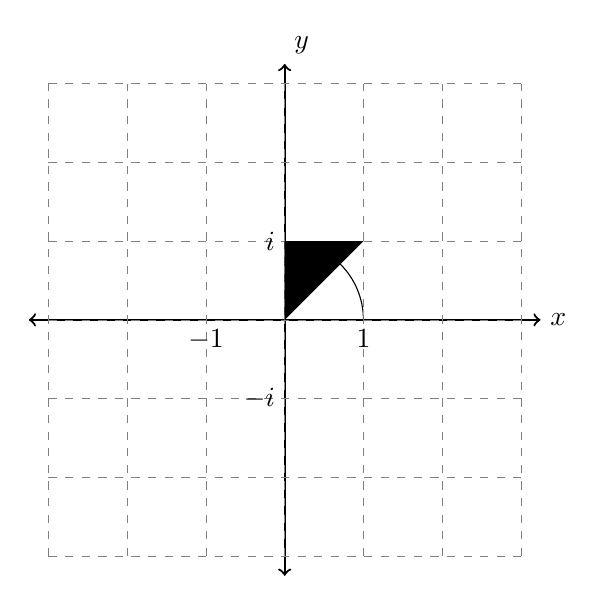
\begin{tikzpicture}[xscale=1, yscale=1]
\draw [thick, <->] (0,-3.25) -- (0,3.25);
\draw [thick, <->] (-3.25,0) -- (3.25,0);
\node [right] at (3.25,0) {$x$};
\node [above right] at (0,3.25) {$y$};
\draw [help lines] [dashed] (-3,-3) grid (3,3);
\node [below ] at (1,0) {$1$};
\node [below ] at (-1,0) {$-1$};
\node [left] at (0,1) {$i$};
\node [left] at (0,-1) {$-i$};
\begin{scope}
    \clip (-1,0) rectangle (1,1);
    \clip (0,-1) rectangle (1,1);
    \draw [fill=white] (0,0) circle(1);
    \draw (-1,0) -- (1,0);
\end{scope}
\draw[dashed] (0,1) -- (1,1);
\fill[fill=black] (0,0)
               -- (0,1)
               -- (1,1)
               -- cycle;
\end{tikzpicture}
$
\hfill
$
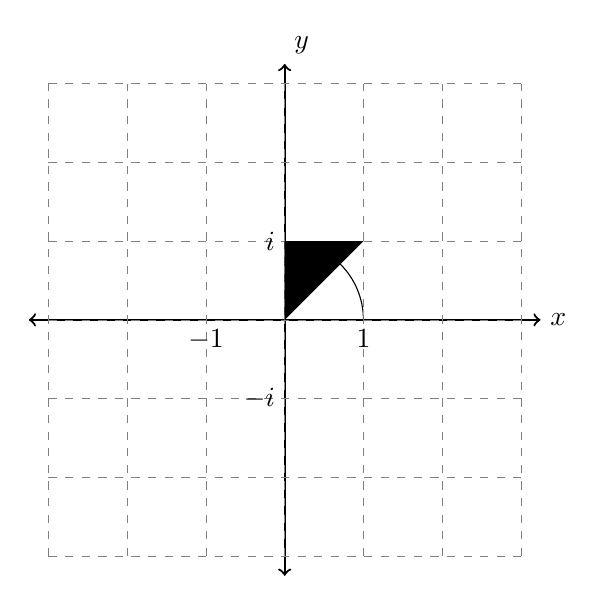
\begin{tikzpicture}[xscale=1, yscale=1]
\draw [thick, <->] (0,-3.25) -- (0,3.25);
\draw [thick, <->] (-3.25,0) -- (3.25,0);
\node [right] at (3.25,0) {$x$};
\node [above right] at (0,3.25) {$y$};
\draw [help lines] [dashed] (-3,-3) grid (3,3);
\node [below ] at (1,0) {$1$};
\node [below ] at (-1,0) {$-1$};
\node [left] at (0,1) {$i$};
\node [left] at (0,-1) {$-i$};
\begin{scope}
    \clip (-1,0) rectangle (1,1);
    \clip (0,-1) rectangle (1,1);
    \draw [fill=white] (0,0) circle(1);
    \draw (-1,0) -- (1,0);
\end{scope}
\draw[dashed] (0,1) -- (1,1);
\fill[fill=black] (0,0)
               -- (0,1)
               -- (1,1)
               -- cycle;
\end{tikzpicture}
$

\noindent \dotfill

\noindent {\bf b.}  the hyperbola $y^2 - x^2=1$ (indicate also orientation)

$
\begin{tikzpicture}[xscale=1, yscale=1]
\draw [thick, <->] (0,-3.25) -- (0,3.25);
\draw [thick, <->] (-3.25,0) -- (3.25,0);
\node [right] at (3.25,0) {$x$};
\node [above right] at (0,3.25) {$y$};
\draw [help lines] [dashed] (-3,-3) grid (3,3);
\node [below ] at (1,0) {$1$};
\node [below ] at (-1,0) {$-1$};
\node [left] at (0,1) {$i$};
\node [left] at (0,-1) {$-i$};
\end{tikzpicture}
$
\hfill
$
\begin{tikzpicture}[xscale=1, yscale=1]
\draw [thick, <->] (0,-3.25) -- (0,3.25);
\draw [thick, <->] (-3.25,0) -- (3.25,0);
\node [right] at (3.25,0) {$u$};
\node [above right] at (0,3.25) {$v$};
\draw [help lines] [dashed] (-3,-3) grid (3,3);
\node [below ] at (1,0) {$1$};
\node [below ] at (-1,0) {$-1$};
\node [left] at (0,1) {$i$};
\node [left] at (0,-1) {$-i$};
\end{tikzpicture}
$

\vskip.1in
\hrule
\vskip.1in

\noindent $\bullet$  The {\sl conjugate transpose} or {\sl Hermitian transpose} of an $m \times n$ complex matrix $A$ is the $n \times m$ matrix $A^H = \overline{A}^T$ obtained from $A$ by taking the complex conjugate of each entry and then taking the transpose. 
\vskip.05in
\noindent $\bullet$ A complex matrix $S$ is a  \emph{Hermitian matrix} if $S=S^H$.

\vskip.1in

\noindent{\bf 2. }  Use properties of the transpose of a matrix and complex arithmetic to prove that  $A^HA$ is always a Hermitian matrix.

\begin{proof}

\end{proof}

\vskip.1in
\hrule
\vskip.1in

\noindent{\bf 3. }  Let $F= \begin{bmatrix}
1 & 1 & 1 & 1 \\
1 & i & -1 & -i \\
1 & -1 & 1 & -1 \\
1 & -i & -1 & i
\end{bmatrix}$
denote the $4 \times 4$ Fourier matrix.  Compute:
\vskip.15in
\noindent{\bf a. } $F^2=
\begin{bmatrix}
* & * & * & * \\
* & * & * & * \\
* & * & * & * \\
* & * & * & *
\end{bmatrix}$
\vskip.15in
\noindent{\bf b. } $F^4=
\begin{bmatrix}
* & * & * & * \\
* & * & * & * \\
* & * & * & * \\
* & * & * & *
\end{bmatrix}$.


\vskip.15in
\hrule

\end{document}